\documentclass[conference]{IEEEtran}
\IEEEoverridecommandlockouts
% The preceding line is only needed to identify funding in the first footnote. If that is unneeded, please comment it out.
%\usepackage{cite}
\usepackage{amsmath,amssymb,amsfonts}
\usepackage{algorithmic}
\usepackage{graphicx}
\usepackage{textcomp}
\usepackage{xcolor}
%\def\BibTeX{{\rm B\kern-.05em{\sc i\kern-.025em b}\kern-.08em
%		T\kern-.1667em\lower.7ex\hbox{E}\kern-.125emX}}

\usepackage{hyperref}
\usepackage{biblatex} 
\addbibresource{refs.bib}

\begin{document}
	
	\title{Analysis on Space Debris Detection and Initial Pose Estimation}

	\author{\IEEEauthorblockN{1\textsuperscript{st} Yvette Espinoza}
		\IEEEauthorblockA{\textit{Software Engineer} \\
			\textit{Northrop Grumman}\\
			Redondo Beach, CA, USA \\
			yespinoz@purdue.edu}
	}

	\maketitle
	
% ------------------------------------------------------------------------------------------------------------
% ~ ~ ~ ~ ~ ~ ~ ~ ~ ~ ~ ~ ~ ~ ~ ~ ~ ~ ~ ~ ~ ~ ~ ~ ~ ~ ~ ~ ~ ~ ~ ~ ~ ~ ~ ~ ~ ~ ~ ~ ~ ~ ~ ~ ~ ~ ~ ~ ~ ~ ~ ~ ~ ~ 
% ------------------------------------------------------------------------------------------------------------
	
	\begin{abstract}
		
		Technological improvements over the past few decades have made space exploration more feasible, but the increase in space activity has also resulted in undesirable space debris that can pose a threat to the safety of space crafts. 
		Space surveillance systems can detect and track large debris, providing space situational awareness that reduces the risk of equipment colliding with debris, but such systems often fail to properly identify smaller debris. The main challenge lies with the uncertainty regarding the debris characteristics, making it difficult to accurately predict the orbit.
		Current detection and tracking of small debris is performed by either using ground based systems, or small satellite constellations to gather information on the debris' characteristics and generate orbit predictions.
		This research project looks at the differences between ground based systems and small satellite constellations, focusing on why the constellations are preferred when considering collision avoidance and active debris removal systems. Sample data is generated from a small satellite equipt with a lidar sensor, then used with a template matching algorithm to obtain an initial pose estimate.

	\end{abstract}

% ------------------------------------------------------------------------------------------------------------
% ~ ~ ~ ~ ~ ~ ~ ~ ~ ~ ~ ~ ~ ~ ~ ~ ~ ~ ~ ~ ~ ~ ~ ~ ~ ~ ~ ~ ~ ~ ~ ~ ~ ~ ~ ~ ~ ~ ~ ~ ~ ~ ~ ~ ~ ~ ~ ~ ~ ~ ~ ~ ~ ~ 
% ------------------------------------------------------------------------------------------------------------

	\section{Literature Review}

		Space exploration, first started in the late 1950's with the USSR's launch of Sputnik I, has become a vital part in current technologies.
		Civilians and government alike have come to rely on space systems, such as GNSS or weather satellites, but the addition of new satellites in an already crowded area is increasing the risk of collisions. 
		This idea was first introduced in 1978 by Kessler, who explained the high density of objects in low Earth orbit (LEO) increases the risk of collisions, and collisions themselves would create more debris that would further increase the collision risk, a scenario commonly referred to as the Kessler Syndrome.
		This scenario was brought back to attention in 2009 with the first recorded collision between between two satellites, Iridium 33 and Cosmos 2251, which at the time produced 1,632 space debris fragments larger than 10 cm \cite{Wang2010AnalysisOD}. These fragments are large enough to be tracked by surveillance systems, such as the Department of Defense’s Space Surveillance Network (SSN), but smaller fragments, referred to as small space debris, are more difficult to detect and track. 
		
		Surveillance networks are catalogs that contain characteristics of registered objects, such as the orbital parameters, which are essential for providing space situational awareness (SSA) \cite{2019_lidar}.
		They rely on both ground based radars and optical telescopes to track the position of the object over time, information that is needed to determine and predict orbits.
		However, applications such as debris collision warning, or active debris removal require information on smaller debris, along with a higher accuracy in orbit determination and prediction, both of which SSN's struggle to provide \cite{2020_ml_approach}.
		

	\subsection{Small Satellite Constellations}
		In an effort to increase the accuracy of space debris orbit detection and predictions, studies were conducted to validate the concept of space based space surveillance. In 1996 the Midcourse Space Experiment satellite was launched with a Space-Based Visible (SBV) sensor, becoming the first demonstration of space-based surveillance that could be valuable to the SSN as an addition to the ground based systems \cite{stokes2000space}. In the following years more satellites, such as the SBSS Block 10 and the Sapphire, have been deployed and shown to provide a more accurate description of the environment  \cite{multi_spacecraft_2016}. 

		Onboard sensors have an unobstructed view of debris, not affected by the weather as optical systems are, and can provide more accurate measurements when processing occurs onboard the spacecraft instead of relying on ground control centers. Since satellites like the SBSS Block 10 validated the benefits of space based surveillance, research has shifted to different applications, such as debris removal or avoidance systems.
		
		Systems that rely on constellations are generally referred to as target-chaser systems, where the target would be the object of interest, and the chaser the spacecraft equipt with different sensors. Some studies have focused on the spacecraft architecture, coordinating between the different spacecraft to track the target \cite{multi_spacecraft_2016}. Other studies focused on pose acquisition and tracking, using template matching algorithms for the initial pose \cite{2017_pose_pca}\cite{OpromollaRoberto2015Upew}, and a combination of different estimation filters for the tracking portion, such as the unscented kalman filter \cite{unscented_kalman}.
		
		
	\subsection{Pose Acquisition}
		\begin{figure}[htbp]
			\centerline{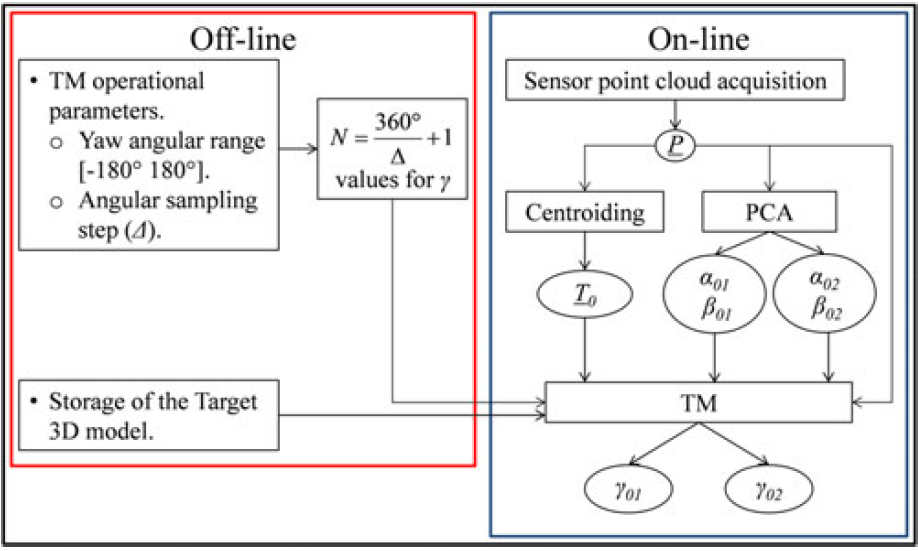
\includegraphics[scale=0.85]{Images/3_D_PCA_based_TM_algorithm.PNG}}
			\caption{3-D PCA-based template matching algorithm.}
			\label{3_D_PCA_based_TM_algorithm}
		\end{figure}
	
		One method for onboard pose determination of space debris involves using a template matching algorithm that processes 3-D point clouds collected from a LIDAR sensor and generates an initial pose measurement, which is later refined using state estimators part of the tracking and orbit estimation \cite{2017_pose_pca}\cite{liu2016point}\cite{unscented_kalman}.
		
		In \cite{2017_pose_pca} the initial pose was defined as 
		
		\centerline{$p_0 = (\alpha_0, \beta_0, \gamma_0, T_0)$}
		
		\noindent where $(\alpha_0, \beta_0, \gamma_0)$ represent the roll, pitch, yaw angles of the debris, and $T_0$ represents the $(x,y,z)$ coordinates. A three step method was proposed to estimate the relative position vector directly from measured point cloud data ($P_c$), referred to as a 3-D PCA-based online Template Matching.
		
		The first step is to obtain the initial position vector ($T_0$) of the target, or debris to track, with respect to the satellite. This is computed as the centroid of the point cloud, shown in equation (\ref{eqn:centroid})).
		\begin{equation}
			\label{eqn:centroid}
			T_0 = -\frac{1}{N} ( \sum_{i=1}^{N} x_i, \sum_{i=1}^{N} y_i, \sum_{i=1}^{N} z_i )
		\end{equation}
		The number of point clouds is given by $N$, with $(x_i, y_i, z_i)$ being points in $P_c$.
		
		After obtaining the initial position vector the main axis ($e_m$) is estimated using the Principle Component Analysis (PCA). From the covariance matrix, calculated from equation (\ref{eqn:covariance}), the main axis directions ($e_{M_x}, e_{M_y}, e_{M_z}$) are obtained from the eigenvector corresponding to the largest eigenvalue of the covariance matrix $Q$. The main axis are used to estimate the roll ($\alpha_0$) and pitch ($\beta_0$) angles, shown in (\ref{eqn:estimated_roll_pitch}).
		\begin{equation}
			\label{eqn:covariance}
			Q = \frac{1}{N} \sum_{i}^{N} (P_c^{(i)} - T_0)(P_c^{(i)} - T_0)^T
		\end{equation}
		
		\begin{equation}
			\label{eqn:estimated_roll_pitch}
			\begin{cases}
				\alpha_0 = tan^{-1}(\frac{e_{M_x}}{e_{M_z}}) \\
				\beta_0 = sin^{-1}(-e_{M_x})
			\end{cases} 
		\end{equation}
	
		The final step is to estimate the yaw angle ($\gamma_0$). This step requires incrementing $\gamma$ and generating a point cloud, or template, of the debris at that angle. The above steps are repeated for each $\gamma$, with an additional step to align the newly calculated and original centroids, then use the nearest neighbor algorithm to determine the similarity between the point clouds. The value of $\gamma$ that minimizes the correlation function is set as the estimated yaw angle.
		
		An overview of the model from acquisition of the point cloud data to the inital pose estimation, taken from \cite{2017_pose_pca} is shown in Figure \ref{3_D_PCA_based_TM_algorithm}.

% ------------------------------------------------------------------------------------------------------------
% ~ ~ ~ ~ ~ ~ ~ ~ ~ ~ ~ ~ ~ ~ ~ ~ ~ ~ ~ ~ ~ ~ ~ ~ ~ ~ ~ ~ ~ ~ ~ ~ ~ ~ ~ ~ ~ ~ ~ ~ ~ ~ ~ ~ ~ ~ ~ ~ ~ ~ ~ ~ ~ ~ 
% ------------------------------------------------------------------------------------------------------------

	\section{Simulation Environment}
		To apply the 3-D PCA template matching algorithm sample data needs to be generated and fed into the algorithm. The sample data was generated in accordance with what was done in \cite{liu2016point}. Their simulated environment takes in a known 3-D model and simulates LIDAR point cloud data that would be collected from an orbiting satellite.


	\subsection{Coordinate System and Pose Parameters}
		Liu, et al \cite{liu2016point}, defines four reference frames, shown in Figure \ref{ReferenceFrames}. The left side shows the chaser, or small satellite $O_c$, which would be equipped with a LIDAR sensor $O_s$. The right side shows the target model $O_m$, which could be any debris of interest, and the model as detected by the LIDAR sensor, $O_t$.
		
		The target model $O_m$ is a point cloud representation of a known 3-D model that is used to estimate the transformation from $O_s$ to $O_m$. In this transformation a point from the target model, $P_m (x_m,y_m,z_m)$ is transformed into a matching point in the sensor frame $P_s (x_s,y_s,z_s)$ through equations (\ref{eqn:T}) - (\ref{eqn:Ps}), where $\phi$ is the rotation about the X-axis, $\theta$ the rotation about the Y-axis, and $\gamma$ the rotation about the Z-axis. 
		
		\begin{equation}
			\label{eqn:T}
			T = \begin{bmatrix} \Delta x  & \Delta y & \Delta z \end{bmatrix}^T
		\end{equation}

		\begin{equation}
		 	\label{eqn:Rx}
			R_X(\phi) = 
			\begin{bmatrix}
				1  & 0 & 0 \\
				0 & cos(\phi) & sin(\phi) \\
				0 & -sin(\phi) & cos(\phi)
			\end{bmatrix}
		\end{equation}
	
		\begin{equation}
			\label{eqn:Ry}
			R_Y(\theta) = 
			\begin{bmatrix}
				cos(\theta)  & 0 & -sin(\theta) \\
				0 & 1 & 0 \\
				sin(\theta) & 0 & cos(\theta)
			\end{bmatrix}
		\end{equation}
	
		\begin{equation}
			\label{eqn:Rz}
			R_Z(\gamma) = 
			\begin{bmatrix}
				cos(\gamma)  & sin(\gamma) & 0 \\
				-sin(\gamma) & cos(\gamma) & 0 \\
				0 & 0 & 1
			\end{bmatrix}
		\end{equation}
	
		\begin{equation}
			\label{eqn:R}
			R = R_Y(\theta) \times R_X(\phi) \times R_Z(\gamma)
		\end{equation}
	
		\begin{equation}
			\label{eqn:Ps}
			P_s = RP_m + T
		\end{equation}
	
	\begin{figure}[htbp]
		\centerline{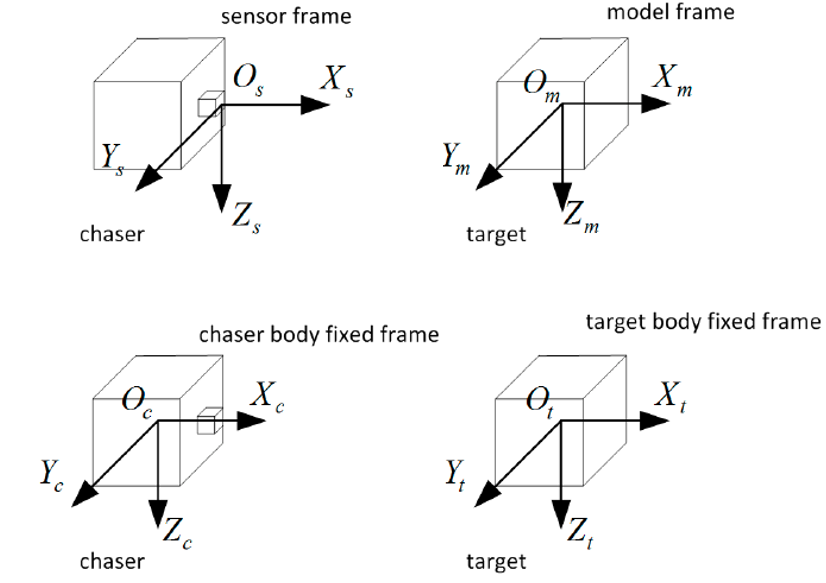
\includegraphics[scale=0.95]{Images/ReferenceFrames.PNG}}
		\caption{Reference frames definition.}
		\label{ReferenceFrames}
	\end{figure}


	\subsection{Target Model}
		Envisat, launched by the European Space Agency in 2002, was initially selected because it appeared in various studies \cite{NocerinoAlessia2021Lmaf}\cite{unscented_kalman}\cite{2017_pose_pca}\cite{OpromollaRoberto2015Upew}. 
		The satellite, which is 26 m (85 ft) × 10 m (33 ft) × 5 m (16 ft) in orbit, was decommissioned and marked as debris after it lost communication in 2012 \cite{envisat_overview}. Though the satellite is very large and does not provide any problems for the ground based SSN to track, its relatively simple shape allow for testing estimation algorithms designed for small satellite constellations.
		
		A 3-D model was obtained online from \cite{envisat_3d_model}, then converted to a point cloud data file. The point cloud data model, shown in Figure \ref{3d_model}, was not to scale, but since the goal of the project was to generate sample LIDAR data and obtain the initial pose estimate, it was deemed suitable for the task.
		\begin{figure}[htbp]
			\centerline{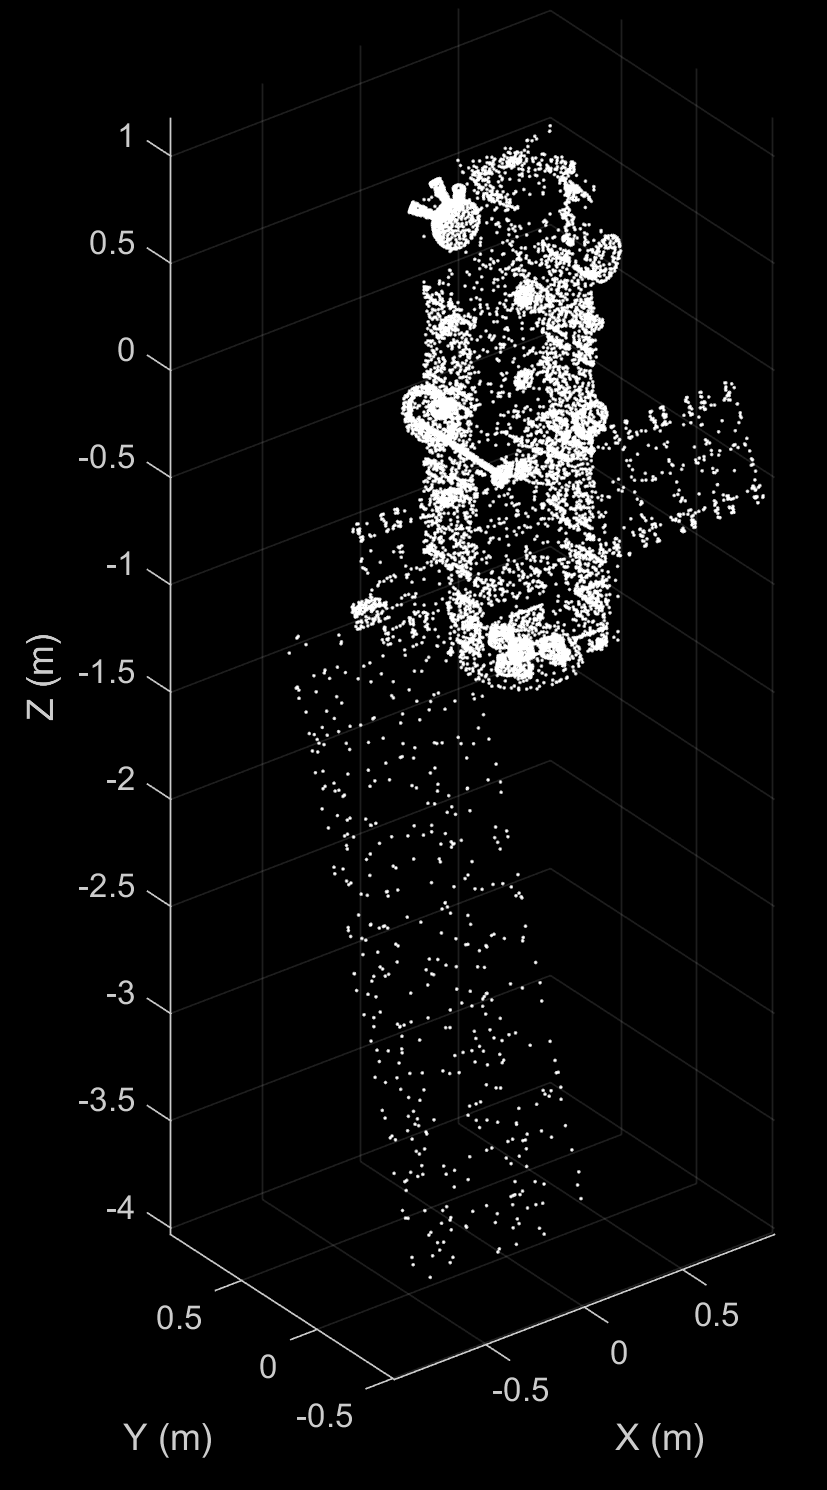
\includegraphics[scale=0.8]{Images/point_cloud_model_black_white.PNG}}
			\caption{ENVISAT 3-D Point Cloud Model.}
			\label{3d_model}
		\end{figure}


	\subsection{Simulated LIDAR Data}
		The SR4000 camera from MESA Imaging was selected as the sensor from which the data is simulated. The specifications were obtained from \cite{camera_specs} and are shown in Table \ref{tab:sr4000_spec}.

		\begin{table}[htbp]
			\caption{SR4000 specifications} %title of the table
			\centering
		\begin{tabular}{rr} % creating 2 columns
			\hline\hline %inserting double-line
			Sensor pixels & 176 x 148 \\ % Entering row contents
			Frame rate & 54 (f/s)\\
			Focus Length ($f$) & 10 (mm) \\
			Scan resolution at 3 m & 13.6 (mm)\\
			Field of view ($\alpha_h,\alpha_v$) & 43.6 x 34.6 (degrees) \\[1ex] % [1ex] adds vertical space
			\hline % inserts single-line
		\end{tabular}
		\label{tab:sr4000_spec}
		\end{table}

		The first step in generating the simulated data was to take the target model point cloud and use equations (\ref{eqn:T}) - (\ref{eqn:Ps}) to get the sensor's view, based on the input rotation angles ($\phi$, $\theta$, $\gamma$), and observed position ($x,y,z$).

		To accurately simulate whether the points lie in the sensors field of view the following equations were used

		\begin{equation}
			\label{eqn:field_view_eqs}
			\begin{cases}
				Y_{range} = \begin{bmatrix} -Dtan(\alpha_h/2), & Dtan(\alpha_h/2) \end{bmatrix} \\
				Z_{range} = \begin{bmatrix} -Dtan(\alpha_v/2), & Dtan(\alpha_v/2) \end{bmatrix}
			\end{cases}
		\end{equation}

		\noindent where $Y_{range}$ and $Z_{range}$ are the horizontal and vertical observable ranges, $D$ is the x component of $P_s$. The horizontal and vertical view angles ($\alpha_h$, $\alpha_v$) are provided in Table \ref{tab:sr4000_spec}. If the calculated sensor point $P_s$ is outside of the sensor range, the point is discarded. To account for distance errors, a random value in the range [$-\Delta d, \Delta d$] was also added.


	% ------------------------------------------------------------------------------------------------------------
	% ~ ~ ~ ~ ~ ~ ~ ~ ~ ~ ~ ~ ~ ~ ~ ~ ~ ~ ~ ~ ~ ~ ~ ~ ~ ~ ~ ~ ~ ~ ~ ~ ~ ~ ~ ~ ~ ~ ~ ~ ~ ~ ~ ~ ~ ~ ~ ~ ~ ~ ~ ~ ~ ~ 
	% ------------------------------------------------------------------------------------------------------------
	\section{Results}
		Matlab was used to take the Envisat 3-D model and convert it to a point cloud file, and Python was used to generate the simulated LIDAR data and obtain the initial pose estimate. The Liu, et al. paper (\cite{liu2016point}) was followed when generating the data, but some assumptions were made when adding the distance measurement errors. The SR4000 camera has a measurement accuracy of 1 cm, but the paper did not discuss how they added their error. The error was assumed to have a Gaussian distribution, zero mean and 1 cm standard deviation, with the error added randomly to one of the three axis.
		
		The code for the project can be found here: \url{https://github.com/Yvette4/AAE575}
		
	\subsection{Experiment 1}
		\begin{figure}[htbp]
			\centerline{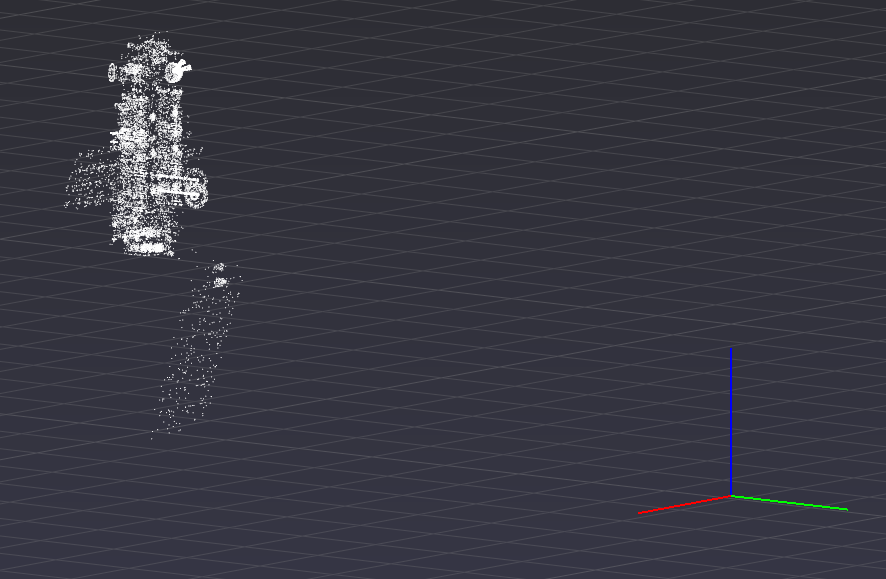
\includegraphics[scale=1]{Images/Experiment1_10m.PNG}}
			\caption{Generated point cloud at 10 meters view distance.}
			\label{Experiment1pc}
		\end{figure}
		The first simulated data was for an observed position (x,y,z) at (10, 0, 0) meters and initial rotation angles ($\phi, \theta, \gamma$) at (-180, 0, 0) degrees. The generated cloud point is shown in Figure \ref{Experiment1pc}.
		
		The following were the initial pose estimates generated:
		\begin{center}
			$T_0 = (-10.012, -0.049,0.200)$
			\[
			\begin{cases}
				\alpha_0 = -13.935 \\
				\beta_0 = 88.818
			\end{cases}
			\]
		\end{center}
		
		The estimated positions were accurate, within centimeters from the true observed position, but the roll and pitch angles were not accurate.
	
		Problems were encountered when estimating the yaw ($\gamma$) angle. The yaw estimate required generating templates of the point cloud data, but the process for generating the template conflicted with how the LIDAR data was being simulated. Due to time constraints the yaw estimate was omitted from the initial pose estimate.

	\subsection{Experiment 2}
	The next observed position was (2, 0, 0) meters and rotation angles (-180, 0, 0) degrees. The generated cloud point is shown in Figure \ref{Experiment2pc}. Since the target was at a close range, the entire model did not fit in the sensor's field of view, which did not detect the bottom panel.
	
	The following is the estimated pose:
	\begin{center}
		$T_0 = (-2.070, -0.066, 0.124)$
		\[
		\begin{cases}
			\alpha_0 = -28.242 \\
			\beta_0 = 86.043
		\end{cases}
		\]
	\end{center}
	
	The estimated pose results were similar to those in experiment 1, with the position estimate within centimeters from the true position, but the roll and pitch angles were not accurate.

	\begin{figure}[htbp]
		\centerline{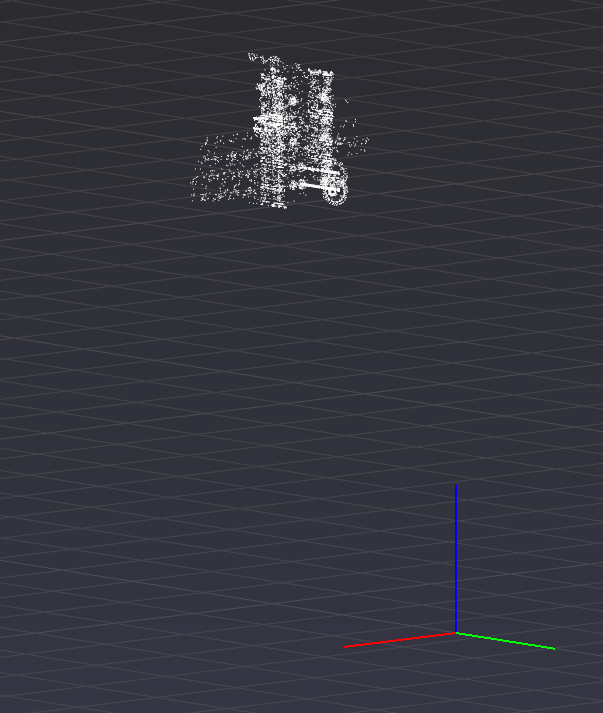
\includegraphics[scale=1]{Images/Experiment2_2m.PNG}}
		\caption{Generated point cloud at 2 meters view distance.}
		\label{Experiment2pc}
	\end{figure}

	\section{Conclusion}
		The LIDAR data was successfully simulated from the provided 3-D target model and the position vector was also successfully estimated with the 3-D PCA template matching algorithm, but the rotation angles were not correct. Due to issues with the template generation portion of the algorithm the yaw estimate was omitted from the calculated pose estimate. Errors in the initial pose estimate are expected as it is only the initial estimate, which would be refined as part of the debris tracking algorithms. 

	\nocite{*}
	\printbibliography
	
\end{document}
